\documentclass{article}
\usepackage{algorithm}
\usepackage{algpseudocode}
\usepackage{amsmath,amssymb,amsthm}
\usepackage{tcolorbox}
\usepackage{booktabs}
\usepackage{a4wide}

\usepackage{tikz}
\usetikzlibrary{trees}
\usepackage{amssymb}
\usepackage{pifont}

\algrenewcommand\algorithmiccomment[1]{\quad// #1}

%TikZ commands
\newcommand*\encircled[1]{\tikz[baseline=(char.base)]{
            \node[shape=circle,draw,inner sep=0.25pt,minimum size=1em] (char) {\vphantom{Ag}#1};}}
\newcommand*\framed[1]{\tikz[baseline=(char.base)]{
            \node[draw,inner sep=0.25pt,minimum size=1em] (char) {\vphantom{Ag}#1};}}

\newtheorem{example}{Example}
\newtheorem{theorem}{Theorem}
\newtheorem{definition}{Definition}
\newtheorem{observation}{Observation}
\newtheorem{proposition}{Proposition}
\newtheorem{conjecture}{Conjecture}
\newtheorem{corollary}{Corollary}
\newtheorem{lemma}{Lemma}

\title{Possible and Necessary Popularity in House Allocation PseudoCode}

\begin{document}

\maketitle

\section{Hypothesis}
\begin{itemize}
    \item Agents give their partial strict linear order (pairwise comparison).
    \item There are as many objects as agents.
    \item We consider only strict linear order.
\end{itemize}

\section{Properties}

\begin{proposition}[Verify Possibly popular matching]
If $\exists i,j \in N$ such that $\sigma(j) P_i \sigma(i)$ and $\exists o \in O$ such that $o \succ_j \sigma(j) $ then return False (the matching is not popular).
\end{proposition}
\begin{proposition}[Find Possibly popular completion]
If $\exists i,j \in N$ such that $\sigma(j) P_i \sigma(i)$ for $o \in O$ such that $(\sigma(j),o) \notin P$ add $(\sigma(j),o) in \succ_j$
\end{proposition}


\begin{proposition}[Find Possibly popular completion - Rewritting]
For a given possibly popular matching on a partial profile $P$, there is a complete completion that can be constructed as follows:
If $\exists i,j \in N$ such that
\begin{itemize}
    \item $\mu(j) P_i \mu(i)$ and for $o \in O \backslash \{\mu(j)\}$ such that $(\mu(j),o) \notin P$ add $(\mu(j),o) in \succ_j$
    \item $(\mu(i), \mu(j)) \notin P_i$, add $(\mu(i),\mu(j)) in \succ_i$
\end{itemize}
\end{proposition}

\begin{proposition}[Find Necessarily popular matching]
If $\exists i,j \in N$ such that $\sigma(j) P_i \sigma(i)$ and $o \in O$
\begin{itemize}
    \item $o P_j \sigma(j)$ or
    \item $(\sigma(j),o) \notin P_j$
\end{itemize}
Return False (it is not a necessarily popular matching).
\end{proposition}
\begin{proposition}[Find Necessarily popular completion]
If $\exists i,j \in N$ such that \\ $(\sigma(i), \sigma(j)), (\sigma(j), \sigma(i)) \notin P_i$ and $o \in O$ such that
\begin{itemize}
    \item $o P_j \sigma(j)$
    \item $(\sigma(j),o) \notin P_j$
\end{itemize}
Return False (it is not a necessarily popular matching).
\end{proposition}

% FAUX
% \begin{proposition}
% If at least half of agents have the same fpost, it is not possible to find a popular matching.
% \end{proposition}


\section{Algorithms}

\subsection{Implementation with pairwise comparison}
\begin{algorithm}[H]
\caption{VerifPossiblyPopularMatching}
\begin{algorithmic}[1]
    \State \textbf{Input:} $O$ the set of n objects, $N$ the set of n agents, $P = (P_1, ..., P_n)$ the partial profile such that $P_i = [(o_l, o_k), ...]$ is the list of pairwise partial preferrence of agent i, $\mu = \{1\colon \sigma(1), ..., n\colon \sigma(n)\}$ is the matching ($\sigma(i)$ is the assigned object to i in the matching). 
    \State \textbf{Output:} boolean indicating either the matching $\mu$ is possibly popular
    \For{each agent $i \in N$}
        \For{each preference $(o_{sup}, o_{inf}) \in P_i$}
            \State NotFpost $\leftarrow o_{inf}$ is $\sigma(i)$
            \State NotDominatedByFpost  $\leftarrow False $
            \For{each preference $(o, o') \in P_j$ }
                \State NotDominatedByFpost $\leftarrow o_{sup}$ is $o'$
            \EndFor
            \If{NotFpost and NotDominatedByFpost}
                \State \Return False
            \EndIf
        \EndFor
    \EndFor
    \State \Return True
\end{algorithmic}
\end{algorithm}

\begin{algorithm}[H]
\caption{FindPossiblyPopularMatching}
\begin{algorithmic}[1]
    \State \textbf{Input:} $O$ the set of n objects, $N$ the set of n agents, $P = (P_1, ..., P_n)$ the partial profile such that $P_i = [(o_l, o_k), ...]$ is the list of pairwise partial preferrence of agent i, $\mu = \{1\colon \sigma(1), ..., n\colon \sigma(n)\}$ is the perfect matching ($\sigma(i)$ is the assigned object to i in the matching). 
    \State \textbf{Output:} A complete completion that making the matching popular.
    \State $\succ$ the complete completion $\leftarrow$ copy of the partial completion $P$
    \For{each agent $i \in N$}
        \For{each objects $sigma(j)$ and agents $j$ matched $\in \mu$}
           \If{$\exists (\sigma(j), \sigma(i)) \in P_i$}
                \For{each objects $o \in O \backslash \{\sigma(j)\}$ }
                    \If{$(\sigma(j), o) \notin P_j$}
                        \State Add $(\sigma(j), o)$ in $\succ_j$
                    \EndIf
                \EndFor
           \ElsIf{$\nexists (\sigma(i), \sigma(j)) \in P_i$}
                \State Add $(\sigma(i), \sigma(j))$ in $\succ_i$
           \EndIf
        \EndFor
    \EndFor
    \State \Return $\succ$
\end{algorithmic}
\end{algorithm}

\subsection{First implementation with positional ranking}

\begin{algorithm}[H]
\caption{VerifPossiblePopularMatching}
\begin{algorithmic}[1]
    \State \textbf{Input:} $O$ the set of n objects, $N$ the set of n agents, $P = (P_1, ..., P_n)$ the partial profile such that $P_i = [?, \sigma(i), o, ...]$ is the list of partial preferrence of agent i (? indicates unknown preference and $\sigma(i)$ is the assigned object to i in the matching), $\mu = \{1\colon \sigma(1), ..., n\colon \sigma(n)\}$ is the matching. 
    \State \textbf{Output:} boolean indicating either the matching $\mu$ is possibly popular, $P$ a completion of the partial profile making $\mu$ possibly popular.
    \State
    \For{each agent $i \in N$}
        \For{each preference $p \in P_i$}
            \If{$p$ is unknown (equal to ?)}
                \State \Comment{Is there a completion such as p is the fpost matched to another agent in $\mu$?}
                \If{$\sigma(i)$ not in $P_i$}
                    \State Assign $\sigma(i)$ to $p$
                \Else
                    \State Find a matched fpost (should not be a fpost for more than half agents) and assigned it to p
                \EndIf
            \ElsIf{$p$ is $\sigma(i)$}
                \State Complete the preference list $P_i$ with the remaining objects.
                \State Break
            \Else
                \State \Comment{$p$ is an object with a better rank than $\sigma(i)$}
                \If{$p$ is a fpost matched to another agent}
                    \State Continue
                \Else
                    \State \Comment{$p$ is not a matched fpost, the matching $\mu$ cannot be popular}
                    \State \Return False, $P$
                \EndIf
            \EndIf
        \EndFor
    \EndFor
    \State
    \Return result
\end{algorithmic}
\end{algorithm}

\begin{algorithm}[H]
\caption{VerifyNecessarilyPopularMatching}
\begin{algorithmic}[1]
    \State \textbf{Input:} $O$, $N$, $P=(P_1, ..., P_n)$, $\mu = \{(1, \sigma(1)), ..., (n, \sigma(n))\}$
    \State \textbf{Output:} boolean indicating either the matching is necessarily popular or not.
    \State $cpt_fpost := 0$
    \For{each $i \in N$}
        \State $Isfpost := True$
        \State \Comment{A matching is popular if each agent obtained either its fpost or spost. }
        \State \Comment{A fpost and/or a spost can not be specified by an agent at the beginning. So we check if all the possible complétion respect this condition.}
        \While{There exist a completion of the agent's i preference list}
            \State $O_i :=$ the set of non ranked item by agent i. 
            \For{Each unknown $p \in P_i$}
                \State Choose an $o$ in $O_i$ for each unknown $p$
                \State $O_i \leftarrow O_i \ \{o\}$
            \EndFor
            \State \Comment{At the end of this for loop, we get a completion of the agent's i preference list}
            \State \Comment{Checking this completion respect the necessarily popular conditions}
            \If{not ($\sigma(i) \in \{f(i), s(i)\}$)}
                \State \Return False;
            \ElsIf{$\exists x \in P_i$ such that $x \succ_i \sigma(i)$ and $x$ not a fpost}
                \State \Return False;
            \EndIf
            \If{$\sigma(i) is not an fpost in this completion$}
                \State $Isfpost \leftarrow False$
            \EndIf
        \EndWhile
        \If{$Isfpost$}
            \State $cpt_fpost \leftarrow cpt_fpost + 1$
        \EndIf
        \State \Comment{If at least half of fpost are assigned, the matching $\mu$ is necessarily popular }
        \If{$cpt_fpost \geq \lceil n/2 \rceil$ }
            \State \Return False;
        \EndIf
    \EndFor
    \State \Return True;
\end{algorithmic}
\end{algorithm}


\section{Examples}

\textbf{Instance for possibly popular matching}
Let H an instance of the House Allocation problem such as:
\begin{itemize}
    \item $N =  \{Alice, Bob, Amelie \}$ the set of agents
    \item $O = \{ a, b, c \} $ the set of objects (houses)
    \item $P = \{P_1, P_2, P_3\}$ the partial profile for which $P_i$ is the strict partial preference order of the agent $i$.
    \item $\mu = \{ (Alice, b), (Bob, c), (Amelie, a)\}$ the matching. Some object specified in the matching are not ranked in some preference lists.
\end{itemize} 
\begin{center}
\begin{tabular}{llllll}
\toprule
\textbf{Agents} & \textbf{$P_i$} & \multicolumn{3}{c}{\textbf{Completions}} \\
\midrule
Alice & ? a ? & $\framed{b}$ $\encircled{a}$ c & $\framed{b}$ a c & c a $\framed{b}$ \\
Bob & b ? ? & $\encircled{b}$ $\framed{c}$ a &  b $\framed{c}$ a & b $\framed{c}$ a \\
Amelie & ? a ? & $\encircled{c}$ $\framed{a}$ b & b $\framed{a}$ a & b $\framed{a}$ c \\
 & & not popular & no solution & not popular \\
\bottomrule
\end{tabular}
\end{center}

\textbf{Instance for necessarily popular matching - Non necessarily popular matching}
Let H an instance of the House Allocation problem such as:
\begin{itemize}
    \item $N =  \{Alice, Bob, Amelie \}$ the set of agents
    \item $O = \{ a, b, c \} $ the set of objects (houses)
    \item $P = \{P_1, P_2, P_3\}$ the partial profile for which $P_i$ is the strict partial preference order of the agent $i$.
    \item $\mu = \{ (Alice, a), (Bob, b), (Amelie, c)\}$ the matching. Some object specified in the matching are not ranked in some preference lists.
\end{itemize} 
\begin{center}
\begin{tabular}{llllll}
\toprule
\textbf{Agents} & \textbf{$P_i$} & \multicolumn{3}{c}{\textbf{Completions}} \\
\midrule
Alice & ? a b & $\framed{b}$ $\encircled{a}$ c & $\framed{b}$ a c & c a $\framed{b}$ \\
Bob & ? ? a & $\encircled{b}$ $\framed{c}$ a &  b $\framed{c}$ a & b $\framed{c}$ a \\
Amelie & c ? ? & $\encircled{c}$ $\framed{a}$ b & b $\framed{a}$ a & b $\framed{a}$ c \\
 & & not popular & no solution & not popular \\
\bottomrule
\end{tabular}
\end{center}


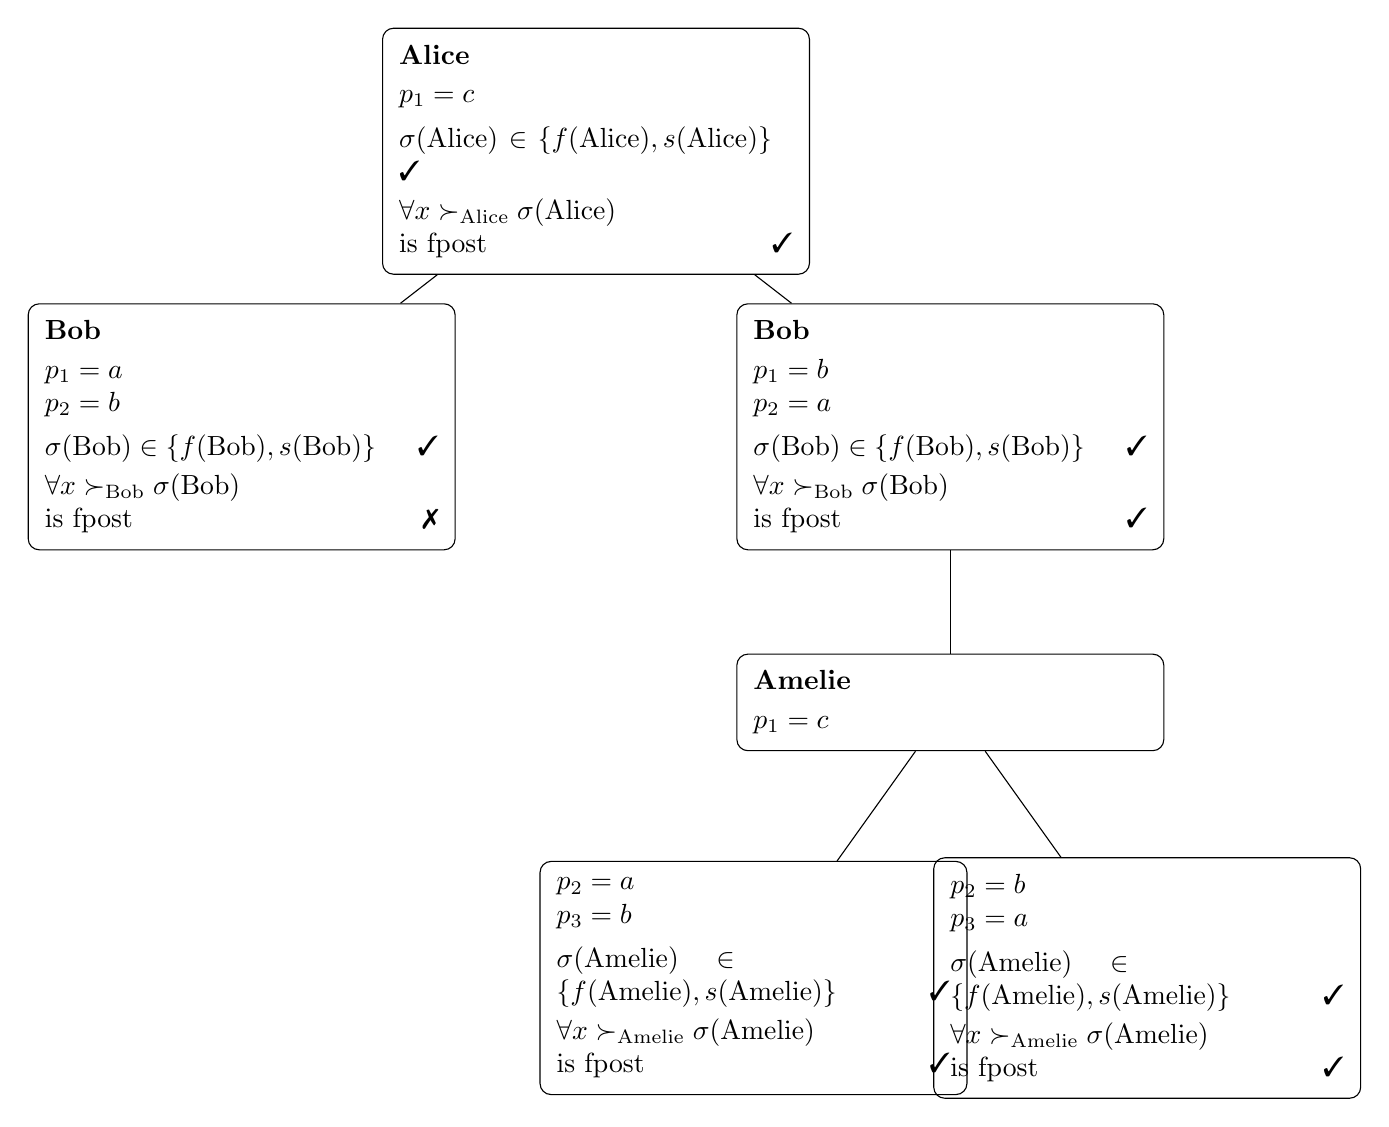
\begin{tikzpicture}[
  level distance=3.5cm,
  level 1/.style={sibling distance=9cm},
  level 2/.style={sibling distance=6cm},
  level 3/.style={sibling distance=5cm},
  every node/.style={
    draw,
    rounded corners,
    align=left,
    text width=5cm,
    inner sep=6pt
  }
]

\node {
\textbf{Alice} \\[2pt]
$p_1 = c$ \\[4pt]
$\sigma(\text{Alice}) \in \{f(\text{Alice}), s(\text{Alice})\}$ \hfill \ding{51} \\[2pt]
$\forall x \succ_{\text{Alice}} \sigma(\text{Alice})$ \\ 
is fpost \hfill \ding{51}
}
child {
    node {
    \textbf{Bob} \\[2pt]
    $p_1 = a$ \\
    $p_2 = b$ \\[4pt]
    $\sigma(\text{Bob}) \in \{f(\text{Bob}), s(\text{Bob})\}$ \hfill \ding{51} \\[2pt]
    $\forall x \succ_{\text{Bob}} \sigma(\text{Bob})$ \\ 
    is fpost \hfill \ding{55}
    }
}
child {
    node {
    \textbf{Bob} \\[2pt]
    $p_1 = b$ \\
    $p_2 = a$ \\[4pt]
    $\sigma(\text{Bob}) \in \{f(\text{Bob}), s(\text{Bob})\}$ \hfill \ding{51} \\[2pt]
    $\forall x \succ_{\text{Bob}} \sigma(\text{Bob})$ \\ 
    is fpost \hfill \ding{51}
    }
    child {
        node {
        \textbf{Amelie} \\[2pt]
        $p_1 = c$
        }
        child {
            node {
            $p_2 = a$ \\
            $p_3 = b$ \\[4pt]
            $\sigma(\text{Amelie}) \in \{f(\text{Amelie}), s(\text{Amelie})\}$ \hfill \ding{51} \\[2pt]
            $\forall x \succ_{\text{Amelie}} \sigma(\text{Amelie})$ \\ 
            is fpost \hfill \ding{51}
            }
        }
        child {
            node {
            $p_2 = b$ \\
            $p_3 = a$ \\[4pt]
            $\sigma(\text{Amelie}) \in \{f(\text{Amelie}), s(\text{Amelie})\}$ \hfill \ding{51} \\[2pt]
            $\forall x \succ_{\text{Amelie}} \sigma(\text{Amelie})$ \\ 
            is fpost \hfill \ding{51}
            }
        }
    }
};
\end{tikzpicture}

\pagebreak


\section{Proof}

\subsection{Proof Verif Possible Popular Matching}

\paragraph{Hypotheses}
\begin{itemize}
    \item $N$ is a set of $n$ agents and $O$ a set of $n$ objects.
    \item We assume a \textbf{perfect matching}: $|N| = |O|$ and all agents/objects are matched.
    \item Preferences are given as \textbf{partial orders} (pairwise comparisons).
    \item We consider \textbf{completions of the partial preference profile}.
    \item $\mu$ is a matching.
\end{itemize}

\paragraph{Definitions}

\begin{itemize}
    \item A \textbf{completion} is a strict complete order extending the partial preferences.
    \item A matching $\mu$ is \textbf{popular} if for every matching $\mu'$:
    \[
    |\{i \in N : \mu(i) \succ_i \mu'(i)\}| \ge |\{i \in N : \mu'(i) \succ_i \mu(i)\}|.
    \]
    \item $\mu$ is \textbf{possibly popular} if it is popular under at least one completion of the partial preference profile.
\end{itemize}


\paragraph{Proof of $\Rightarrow$}

Suppose that there exist $i,j \in N$ such that
\[
\sigma(j) P_i \sigma(i)
\quad \text{and} \quad
\exists o \in O \text{ such that } o \succ_j \sigma(j).
\]

We prove that $\mu$ is not possibly popular.

Let $\succ$ be any completion of the partial preference profile $P$. We show that $\mu$ is not popular under $\succ$ by constructing a matching $\mu'$ that defeats $\mu$.

\medskip

\textbf{Construction of $\mu'$}

\begin{itemize}
    \item If $o$ is unmatched in $\mu$, define:
    \[
    \mu'(i) = \sigma(j), \quad \mu'(j) = o.
    \]
    
    \item Otherwise, there exists $k \in N$ such that $o = \sigma(k)$. Define a local exchange:
    \[
    \mu'(i) = \sigma(j), \quad
    \mu'(j) = o, \quad
    \mu'(k) = \sigma(i),
    \]
    and for all $\ell \notin \{i,j,k\}$:
    \[
    \mu'(\ell) = \mu(\ell).
    \]
\end{itemize}

\medskip

\textbf{Validity}

The matching $\mu'$ is valid since it corresponds to a permutation of objects among at most three agents and leaves all others unchanged.

\medskip

\textbf{Comparison of $\mu$ and $\mu'$}

\begin{itemize}
    \item Agent $i$ prefers $\mu'$:
    \[
    \sigma(j) \succ_i \sigma(i).
    \]
    
    \item Agent $j$ prefers $\mu'$:
    \[
    o \succ_j \sigma(j).
    \]
    
    \item At most one agent (namely $k$ if it exists) may prefer $\mu$.
    
    \item All other agents are indifferent.
\end{itemize}

\medskip

\textbf{Vote count}

\[
|\{i \in N : \mu'(i) \succ_i \mu(i)\}| \ge 2
\quad \text{and} \quad
|\{i \in N : \mu(i) \succ_i \mu'(i)\}| \le 1.
\]

Thus, $\mu'$ is more popular than $\mu$, contradicting the popularity of $\mu$.

\medskip

Since this holds for any completion, $\mu$ is not possibly popular.

\qed


\paragraph{Proof of $\Leftarrow$}

Suppose that $\mu$ is not possibly popular. Then for every completion of the partial preference profile, $\mu$ is not popular.

We use the following characterization from Abraham et al.:

\medskip

\textbf{Lemma (Abraham et al.)}  
A matching $\mu$ is popular if and only if:
\begin{itemize}
    \item every agent is matched to either its $fpost$ or its $spost$,
    \item and every $fpost$ is matched.
\end{itemize}

\medskip

By contraposition of the lemma (Abraham et al), since $\mu$ is not popular for any completion, for every completion there exists at least one agent $i$ such that:
\[
\mu(i) \notin \{fpost(i), spost(i)\}.
\]

In particular, this implies:
\[
fpost(i) \succ_i \mu(i).
\]

Let $j \in N$ be such that:
\[
\mu(j) = fpost(i).
\]

Thus:
\[
\sigma(j) \succ_i \sigma(i).
\]

Let $k \in N$ be such that:
\[
\mu(k) = spost(i).
\]

We distinguish the following cases:

\begin{enumerate}
    \item If $\mu(j) \notin \{fpost(j), spost(j)\}$, then by definition of $fpost(j)$ there exists an object $o \in O$ such that:
    \[
    o \succ_j \mu(j),
    \]
    and the property holds.

    \item If $\mu(j) = spost(j)$, then by definition of $fpost(j)$ we have:
    \[
    fpost(j) \succ_j \mu(j),
    \]
    so there exists $o = fpost(j)$ such that:
    \[
    o \succ_j \sigma(j).
    \]

    \item If $\sigma(j) = fpost(j)$ and $\sigma(k) = fpost(k)$, then both agents receive their $fpost$.

    Since $\mu$ is assumed not popular, this contradicts the characterization of Abraham et al., which requires that every agent is matched to either its $fpost$ or $spost$, and that every $fpost$ is matched. Hence, this situation cannot occur under our assumption.

\end{enumerate}

\medskip

In all cases, we obtain:
\[
\exists o \in O \text{ such that } o \succ_j \sigma(j).
\]

\medskip

Therefore:
\[
\exists i,j \in N \text{ such that } \sigma(j) \succ_i \sigma(i)
\quad \text{and} \quad
\exists o \in O \text{ such that } o \succ_j \sigma(j).
\]

This proves the desired property.

\qed

\subsection{Proof Find Possibly Popular Completion}

\paragraph{Hypotheses}
\begin{itemize}
    \item $N$ is a set of $n$ agents and $O$ a set of $n$ objects.
    \item We assume a \textbf{perfect matching}: $|N| = |O|$ and all agents/objects are matched.
    \item Preferences are given as \textbf{partial orders} (pairwise comparisons).
    \item We consider \textbf{completions of the partial preference profile $P$} $\succ$.
    \item $\mu$ is a possibly popular matching.
\end{itemize}

\paragraph{Definitions}
\begin{itemize}
    \item $\forall i \in N, \forall o \in O \backslash \{\sigma(i)\}$, $\exists (\sigma(i), o)$ or $(o, \sigma(i))$ in $\succ_i$.
    \item \textbf{From Handbook of Computational Social Choice (p26):} $a \gtrsim b$ or $b \gtrsim a$ for all $a \neq b \in O$ and any voter $i \in N$
    \item \textbf{Szpilrajn's Theorem:} Any partial order extends to a total order.
\end{itemize}

\paragraph{Proof}
% We suppose $\mu$ is a possibly popular and perfect matching. 
% Suppose we have found a completion that makes $\mu$ popular such that $\exists i,j \in N$:
% \begin{itemize}
%     \item if $\sigma(j) P_i \sigma(i)$ and for $o \in O$ such that $(\sigma(j), o) \notin P_j$ then $(\sigma(j), o) \in \succ_j$
%     \item if $(\sigma(i), \sigma(j)) \notin P_i$ then $(\sigma(i), \sigma(j)) \in \succ_i$
% \end{itemize}
% Let's prove that this completion is indeed complete and that $\mu$ is a popular matching under this completion.\\
% \textbf{Intuition:}
% $O$ is the set of all objects and because $\mu$ is a perfect matching, $O$ contains all the matched objects. 
% So we can rewritte $O$ as $O = \{\sigma(k) : k \in N\}$.
% For each object $\sigma(k) \in O \backslash \{\sigma(i)\}$ and for each agent $i \in N$,
% \begin{itemize}
%     \item either $(\sigma(i), \sigma(k)) \in \succ_i$
%     \item or $(\sigma(k), \sigma(i))$ and $(\sigma(k), o) \in \succ_j$ for all $o \in O$
% \end{itemize}






From the definition of a possibly popular matching $\mu $, we know that there exists a completion $\succ$ of the partial preference profile $P$ such that $\mu$ is popular under $\succ$.
Under this completion and from the Abraham et al. characterization of popular matchings, we have that every agent is matched to either its $fpost$ or its $spost$, and every $fpost$ is matched.
Hence:
\begin{enumerate}
    \item Because there are as many agents as houses, for all agent $i \in N$, $\mu(i)$ is a $fpost$ of any agent $j$ such that $fpost(j) \succ_i o$ for all houses $o \in O \backslash \{fpost(j)\}$.
    \item For all $\mu(i)$, if there does not exist an agent $j$ such that $\mu(i) = fpost(j)$, then $\mu$ is not popular under $\succ$, which is a contradiction of the second condition of the characterization of Abraham et al.
    \item For all $\mu(i)$, if $\mu(i) \succeq_i spost(i)$ then the first condition of the characterization of Abraham et al. is verified. In the other case, when $spost(i) \succ_i \mu(i)$, the first condition is not verified and $\mu$ is not popular under $\succ$.
\end{enumerate}

Reasoning with these three points, we are looking to reconstruct a completion $\succ$ from the partial preference profile $P$.

Let's prove that the construction is well-defined by showing that:
\begin{enumerate}
    \item The obtained completion is composed of strict linear orders over the set of all houses and it is irreflexive (no ties), asymmetric and transitive.
    \item The obtained completion is a total linear order. Each agent $i$ has a complete preference list over all houses $O$, i.e. for all agent $i \in N $ there exists a relation $\succ_i$ such that for all $o, o' \in O$, either $o \succ_i o'$ or $o' \succ_i o$.
    \item The obtained order is transitive. For all agent $i \in N$, for all $a, b, c \in O$, if $a \succ_i b$ and $b \succ_i c$ then $a \succ_i c$.
    \item The completion should be consistent with the partial preference profile $P$.
    \item The completion does not have any cycle. For all agent $i \in N$, for all $a, b, c \in O$, if $a \succ_i b$ and $b \succ_i c$ then not $c \succ_i a$.
\end{enumerate}


\textbf{1. Strict linear order}

We work with \emph{strict} linear orders, consistently with the partial preference profile $P$.


Irreflexitivity means that no house is in relation with itself, i.e. for all $i \in N$ and for all $o \in O$, $(o, o) \notin succ_i$.
For all $i \in N$ and for all $o, o' \in O$ such that $(o', o) \notin P_i$: 
if $o=o'$, then $(o, o') \notin \succ_i$ because our construction rules do not add any relation between $o$ and itself.
Otherwise the irreflexivity is verified because the relation is not between $o$ and itself.


Asymmetry does not allows to a house $o$ preferred to another $o'$ to be also less preferred than $o'$, i.e 
for all $i \in N$ and for all $o, o' \in O$ $(o \neq o')$ such that $(o, o') \in \succ_i$ then $(o', o) \notin \succ_i$.
if $o = \sigma(i)$ and $o' = \sigma(j)$ and $(\sigma(i), \sigma(j)) \notin P_i$, then $(o, o') \in \succ_i$. 
By contradiction, let's suppose that $(\sigma(j), \sigma(i)) \in \succ_i$. 

\textbf{$=>$ Need to rewrite the proposition!}



\textbf{Sources:}
\begin{itemize}
    \item https://fr.wikipedia.org/wiki/Th%C3%A9or%C3%A8me_d%27extension_de_Szpilrajn
\end{itemize}



% =>

% Suppose for a contradiction that the matching $\mu$ is popular for a given completion and $\exists i,j \in N$ such that $\sigma(j) P_i \sigma(i)$ and $\exists o \in O$ such that $o \succ_j \sigma(j) $.
% Given the lemma 2.4 describe in the paper "Popular Matching" of Abraham et al, a matching is popular if and only if each agent is matched either with its fpost or its spost and every fpost is matched.

% \begin{itemize}
%     \item The agent i is not matched to its fpost because $\sigma(j) \succ_i \sigma(i)$. So agent i will be matched to its spost and agent j will be matched to the fpost of i.
%     \item The agent j is not matched to its fpost because $\exists o \in O$ such that $o \succ_j \sigma(j) $. So agent j will be matched to its spost and $o$ is its fpost.
%     \item Let $\mu'$ be another matching such that $\sigma'(i) = fpost(i) = \sigma(j)$ and $\sigma'(j) = fpost(j) = o$. So agents i and j will prefer $\mu'$ to $\mu$ and by consequence, $\mu'$ is more popular than $\mu$. It is a contradiction because we have assumed that $\mu$ is popular.
% \end{itemize}
% To conclude, this proves the lemma.

% <=
% Suppose that the matching $\mu$ is not popular.
% So $\exists i \in N$ such that $\sigma(i) \notin \{fpost(i), spost(i)\}$. 
% By consequence, $\exists j,k \in N$ such that $\sigma(j) = fpost(i)$ and $\sigma(k) = spost(i)$.
% \begin{enumerate}
%     \item Either $\sigma(j) = fpost(j)$ and $\sigma(k) = fpost(k)$. It is a contradiction because $\mu$ is not popular ($|\{i\in N: \sigma(i)\succ_i \sigma'(i)\}| < |\{i\in N: \sigma'(i)\succ_i \sigma(i)\}|$).
%     \item Either one of them, e.g k gets its fpost and j is matched with its spost. So $\exists o \in O$ such that $o \succ_j \sigma(j)$ and $\sigma(j) \succ_i \sigma(i)$. The property is verified.
%     \item Either one of them, e.g k gets its fpost and $\sigma(j) \notin \{fpost(j), spost(j)\}$. So $\exists o \in O$ such that $o \succ_j \sigma(j)$ and $\sigma(j) \succ_i \sigma(i)$. The property is verified.
% \end{enumerate}
% This proves the reciprocity lemma.


% Let's try to prove this lemma by contradiction.
% Supposing the property \textbf{Prop:} $\exists i,j \in N$ such that $\sigma(j) P_i \sigma(i)$ and $\exists o \in O$ such that $o \succ_j \sigma(j) $ is true. 
% From this property, we assume the matching $\mu$ not possibly popular.

% A matching $\mu$ is possibly popular if it is popular in at least one completion of the partial preference profile.
% \paragraph{Initialization}
% For 2 agents and 2 objects:
% \[
% i: \sigma(j) P_i \framed{$\sigma(i)$}
% \]
% \[
% j: \sigma(i) P_j \framed{$\sigma(j)$}
% \]
% $\exists \mu' = \{(i, \sigma(j)),(j, \sigma(i))\}$ such that $|\{i\in N: \sigma(i)\succ_i \sigma'(i)\}| < |\{i\in N: \sigma'(i)\succ_i \sigma(i)\}|$ (0 $<$ 2).
% Hence $\mu$ is not a popular matching whatever the completion (there are only two possible completions for this setting) for 2 agents and 2 objects.
% \paragraph{Inheritance}
% We suppose the property Prop true for n agents and n objects and we want to determine whether the property is still true for n+1 agents and n+1 objects.
% If $\mu$ is not popular at rank n, this means there is no completion such that $|\{i\in N: \sigma(i)\succ_i \sigma'(i)\}| \geq |\{i\in N: \sigma'(i)\succ_i \sigma(i)\}|$.
% Let's add an agent and an object:
% By contraposition, we have
% \[
% A => B
% \]
% \[
% not B => not A
% \]
% where\\
% B: $\forall$ completions over $n+1$, $\mu$ is not popular.\\
% A: $\forall$ completions over $n$, $\mu$ is not popular.\\
% not B: $\exists$ a completion over $n+1$, such that $\mu$ is popular.\\
% not A: $\exists$ a completion over $n$, such that $\mu$ is popular.\\

% In other words, if we suppose there exists a completion over $n+1$ such that $\mu$ is popular, then this implies that there exists a completion over $n$ such that $\mu$ is popular. 
% However, we said that $\mu$ is not popular over $n$ so all completions over $n+1$ make $\mu$ not popular.\\
% Nevertheless, we must show that if $\exists$ a completion over $n+1$ such that $\mu$ is popular then its restriction over $n$ is still popular.

% Over $n+1$: $|\{i\in N: \sigma(i)\succ_i \sigma'(i)\}| \geq |\{i\in N: \sigma'(i)\succ_i \sigma(i)\}| \forall \mu'$
% We restreint by removing 1 agent and 1 object (called agent k and object k):
% \begin{enumerate}
%     \item agent k $\in \{i\in N: \sigma(i)\succ_i \sigma'(i), \forall \mu'\}$ and object k is not $\sigma(k)$
%     \item agent k $\in \{i\in N: \sigma(i)\succ_i \sigma'(i), \forall \mu'\}$ and object k is $\sigma(k)$
%     \item agent k $\in \{i\in N: \sigma'(i)\succ_i \sigma(i), \forall \mu'\}$ and object k is not $\sigma(k)$
%     \item agent k $\in \{i\in N: \sigma'(i)\succ_i \sigma(i), \forall \mu'\}$ and object k is $\sigma(k)$
% \end{enumerate}


\end{document}